%!TEX root = ../template.tex
%%%%%%%%%%%%%%%%%%%%%%%%%%%%%%%%%%%%%%%%%%%%%%%%%%%%%%%%%%%%%%%%%%%%
%% chapter10.tex
%% NOVA thesis document file
%%
%% Chapter with lots of dummy text
%%%%%%%%%%%%%%%%%%%%%%%%%%%%%%%%%%%%%%%%%%%%%%%%%%%%%%%%%%%%%%%%%%%%

\typeout{NT FILE chapter10.tex}%

\chapter{Conclusion}
\label{cha:Conclusion}


In this work we contemplated fundamental topics of time series data mining. We motivated these topics considering the need for tools that help analysts to better understand what happened during the recording process and find relevant instances on signals that can be related with specific occurrences in the physical world. These motivations are intrinsically related with tools that are more visually interpretable and search mechanisms that are more expressive and intuitive. The work developed highly contributed to each of these domains with relevant standard mechanisms that can be further developed into practical tools for real scenarios. Not only these tool can be practical, but the methods presented bring novelty into the state of the art, either by "borrowing" more traditional methods from other domains (such as the \gls{ssm} in audio information retrieval or \gls{nlp} techniques for text mining) or by introducing novel concepts, specially in terms of text representation of time series and text-based query search mechanisms.
\par
In this Chapter, we highlight the main contributions of this thesis in each of this domains. Comments are also given regarding the contributions and applicability to occupational health scenarios. Finally, overall scientific production and collaborations during the period of this thesis are also provided. 

\section{Main Contributions on General Topics}

As we mentioned in Chapter \ref{cha:introduction}, this thesis would contribute to three main topics, namely \textit{Sensing}, \textit{Analysis} and \textit{Decision Making}:
\begin{itemize}
\item \textit{Sensing:} In this context, a deep understanding of the existing technology to record biosignals was made. At some point, the focus moved towards technology existing to monitor occupational variables. A written work is available regarding the usage of fiber-optics for the monitoring of motion and postural variables in automotive industries, which can be found in \cite{fiber_optics} and it is compared to other existing methods. In addition, a study of the state of the art sensors existing on the market was made to understand the fit in the occupational health problematic. A presentation is available at \cite{sensors_slides}, showing the existing materials on the market and that cover human motion and physiology, more focused for occupational health. The contributions in this area are more related with the knowledge gained and how it was used to more appropriately prepare an acquisition plan regarding the acquisition of occupational variables in several settings, namely automotive industry (Volkswagen Autoeuropa), clothing manufacturers and office/desk jobs.\\

\item \textit{Analysis:} In terms of analysis, the contributions are more practical and relevant. These include the usage of the \gls{ssm} for the segmentation of time series (\textit{novelty} and \textit{periodic}), summarization and creation of similarity profiles for (semi-)automatic clustering. A novel symbolic representation of time series was introduced, and examples were provided in how to apply it for pattern search with \gls{regex} (\gls{ssts}) and text-based classification (\gls{hearts}. A novel search mechanism was also developed, closer to natural language search, with keywords and operators (\gls{quots}). A more detailed explanation of these contributions are provided on a further section.\\

\item \textit{Decision Making:} The main purpose of the studied and developed methods was to help analysts when inspecting time series for several tasks, but also move towards democratizing pattern search on time series. The proposed strategies provide several levels of understanding and help in several layers of decision making. Of course it will depend on the purpose, context, output delivered by the method and the category of expertise of the analyst.
\par
Starting with the analysis of structural information with the \gls{ssm}, it provides a visual output that has characteristic structures that will appear independently of the type of data or context. The main structures will always be blocks, paths and similarity. Being very characteristic, the meaning will always be the same. As we have seen, these can help the analyst identify specific occurrences on time series. Therefore, by learning how to read the \gls{ssm}, more awareness is given to the analyst and more conscious decisions can be made based on that information.
\par
In a standard perspective, the analyst can also perform automatic or semi-automatic segmentation and labeling/annotation of data to accelerate the preparation process to train supervised machine learning algorithms. This can either be done with the visual support of the \gls{ssm} or the supporting methods.
\par
Regarding the process of pattern search with more expressive queries, we believe the tools provide valuable resources to both the analyst that works in the time series domain and is experienced in the computer science field (e.g. a researcher that develops machine learning methods for human activity recognition), and the analyst that is not an expert in computer science but has knowledge in a specific domain of time series (e.g. a physician that is experienced in \gls{ecg} data). In this case, the process is more interactive and requires writing a \gls{regex}/text query. This should be useful to accelerate the search process by an experience computer scientist, because it should be more quick to make the search with this system than developing an algorithm for that purpose. In addition, it contributes to democratize the search mechanism to more analysts than computer scientists, because if the analyst is able to describe the shape being searched, it should be possible to find it (considering the right connotation methods/word feature vectors are used). In that aspect, the information retrieval would very quickly help the analyst in taking more informed decisions.
\end{itemize}


\section{Scientific Contributions}

\subsection{Unveiling the \textit{Grammar} of Time Series}

One of the major topics of this work regarded the segmentation of time series into smaller segments, based on novelty and periodicity. In addition, it was also discussed the benefit of relating the resulting subsequences by how similar these are. As an example, we showed the \gls{abp} signal \vstretch{0.6}{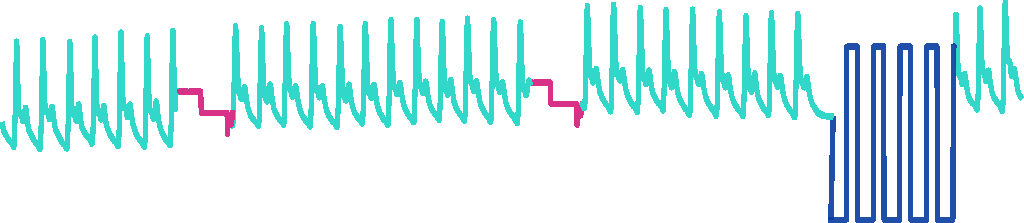
\includegraphics[width=25ex, valign=m]{bvp_thumbnail_final.pdf}}, which can be divided into 7 segments, having the structure \textcolor{mygreen3}{A} \textcolor{mymagenta}{B} \textcolor{mygreen3}{A} \textcolor{mymagenta}{B} \textcolor{mygreen3}{A} \textcolor{myblue5}{C} \textcolor{mygreen3}{A}. We demonstrated with strong evidences that the usage of the \gls{ssm} is reliable in performing this type of task. From the \gls{ssm}, the novelty function can be extracted and the similarity profiles can be compared to perform a segmentation and association between subsequences. In addition, the segmentation might be periodic, meaning that a signal, such as 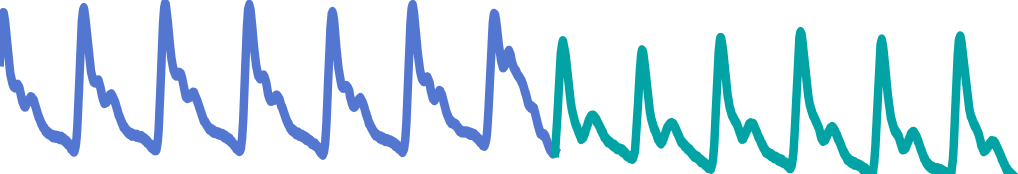
\includegraphics[height=2.5ex, valign=m]{bvpABpng.png}, can be separated into \textcolor{myblue}{A} and \textcolor{mygreen}{B}, but also, \textcolor{myblue}{AAAAAAA}\textcolor{mygreen}{BBBBBB}. We also demonstrated that using the \gls{ssm}, we can compute the similarity function, which highlights the cyclic nature of the subsequence.
\par
The performance of the method was validated for the novelty segmentation  process. It was compared to several SOA methods, showing to be competitive in tasks related with change point detection and segmentation. In addition, several use-cases from various fields were presented as examples, showing the ability of the algorithm to be agnostic to the type of signal, being functional in multidimensional signals and not requiring any previous knowledge on the data, such as the number of segmentation points. It also shows potential to be used for unsupervised annotation of data, being developed towards this purpose.
\par
In this work, datasets were carefully chosen to cover as much real scenarios as possible. Also, common benchmarks were used to validate the methods to guarantee independence from private datasets. Besides, the proposed method was also demonstrated to work well with multimodal and multidimensional occupational data.
\par
There are still several improvements to be made, namely considering the excessive memory that is required to compute the \gls{ssm} in cases where the signal is very large. The fact that a matrix has to be computed limits the ability to analyze in one run the entire signal. This process is specially relevant for periodic segmentation and computing similarity profiles. As previously explained, for novelty segmentation, the process can be adapted to only compute the \gls{ssm} along the diagonal with the size of the kernel width. An adaptation of the process has not yet been presented for the other processes, but a solution should be considered in the future. An additional limitation is the fact that the method is not invariant to trend. If events occur in slow trend changes, that is, a continuous change, the method will have more difficulty in identifying the segmentation point. The usage of pre-processing, additional time series representations, or time series decomposition methods could help in counteracting this effect. Currently, no pre-processing is made to the data. Additional methods could be performed to optimize the process, such as feature reduction and feature stacking.
\par
The ability of the method to be adapted in Online scenarios has not been discussed, but a solution should also be considered in the future.

\subsection{Using Language for Time Series Data Mining}

Representing data into different data types provides a new look on the original data. It may lead to find segments of interest that were not visible in the original data type and/or may benefit from the large experience in mining on this new data type. These are the first arguments for the ideas we presented in this work in transforming time series from the numerical domain to the text/symbolic domain. A new look on time series is possible, which enables to adapt some of the existing data mining techniques with a textual approach, and it can benefit from the large knowledge on text processing or \gls{nlp}.
\par
As a first concept, language and time series can apparently be a strange combination. However, we provided additional evidence that there is a bridge and a potential to perform several tasks with success, namely in text-based query pattern search with \gls{ssts} and \gls{quots}, as well as classification with \gls{hearts}. 
\par
The concept of symbolic representation has started with \gls{sax}, which was a great inspiration for the work developed further with \gls{ssts}. We developed this method with the purpose of making pattern search with more expressive queries, more closely related with the way we look and interpret visually the existing shapes on time series. Several examples were provided showing the possibility of using \gls{regex} (text patterns) on time series symbolic representation. There is still room to improvement. In one end, \gls{regex} are very useful and can be used to design patterns to be searched, but in the other end, \gls{regex} patterns can be very complex and limited to express the textual patterns that are being searched, and the search process is very radical and brittle, in the sense that if the time series patterns do not match the \gls{regex}, no output will be given and the pattern will not be find. In this case, there is no distance measure that is continuous and this should be taken into consideration in a next iteration of the method. Additionally, having higher levels of representation could be useful to search for increasingly higher-leveled structures, such as \texttt{peaks}, \texttt{plateaus} or a combination of these. This idea was what led us perform the next method for time series classification, \gls{hearts}. 
\par
We imagined that if time series could be \textit{translated} into text documents, these could be differentiated based on the words and sentences that would represent them. Inspired by \gls{nlp} techniques used for this purpose, such as \gls{bow} and \gls{tfidf}, we performed classification of time series documents, by creating a high-leveled distance measure that relies in the presence of structures, such as \texttt{peak}, \texttt{plateau}, \texttt{up, down} and \texttt{flat}, etc... and the order of these words in a sentence with ngrams. We then showed that it was possible to use traditional \gls{nlp} methods to perform this task on the UCR classification benchmark. It was able to have a better performance than the 1-NN \gls{ed} and showed to be competitive in this field. Especially because there is the possibility of extracting valuable information from the textual translation, namely by using the \gls{tfidf} weights to highlight areas of relevance on the signal or keywords that mostly represent the topic of the signal (such as topic modeling on text domain). We believe we introduced a novel idea with these processes that can be helpful for search but also for explaining which are the differences between signals. There is still a lot to improve, since as we showed, it would only be interpretable for time series with simple characteristics explained by the \textit{connotation} and \textit{queries} developed and used to describe the signals.
\par
Having queries closer to the way we express what we see was one of the main motivations of this work. This led to the development of \gls{ssts} in the symbolic domain, but we believe as well that features are a good match to specific words that we used to describe parts of signals. This led to the development of \gls{quots}, which uses word-feature vectors to search for specific subsequences on time series by how well these match the set of keywords used, similarly to how we type keywords on \textit{Google} to search for web pages. We provided evidence of its usage in several types of signal and with several types of problems, from motion gestures, to \gls{ecg} patterns or telemetry data, in multidimensional time series. We highlight the potential to use this method to search subsequences based on visual intuition but also for \textit{words} that are \textit{known}, namely by \textit{puppeteering} or \textit{mimicking} shapes in practice. This is specially relevant if keywords can be transformed for each domain, being domain specific. Considering that the vocabulary can change from domain to domain, for instance, \texttt{peak} in medicine can mean an \gls{ecg} peak, while in automotive telemetry, it might mean \textit{turn right}. This domain specific match can help other non-experienced analysts to use it to search for specific patterns.

\section{Other Contributions}

\subsection{Managing Rotation Plans with Exposure, Diversity and Team Homogeneity}

In close collaboration with Volkswagen Autoeuropa and the Faculty of Human Motricity of Lisbon (FMH), we developed a method to automatically suggest job rotation schedules based on ergonomic standards available at the factory. These standard factors are from the AutoErgo tool, based on \gls{eaws} measures. The motivation for the development of such a tool was to help team leaders to manage job rotation schedules more quickly and in a more informed way. Team leaders organize the working schedule for their team by assigning each worker to a sequence of workstations for the entire week, which is a time consuming tasks and not always informed in the risk level that each tasks represents for a worker. In this method, risk exposure, diversity in exposure, as well as team homogeneity, are taken into consideration when suggesting a daily rotation plan. The process was made by developing a genetic based optimization algorithm that followed an objective function developed by our team. The motivation, algorithm and results can be seen at \cite{jobrotation1}.

\subsection{MicroErgo - Concept for Personal Assessment of Occupational Risk in Desk/Office Jobs}

A lot of focus has been given to occupational health scenarios during my thesis. Especially for the main projects in which the group was involved. One of these projects is \gls{prevoccupai}, which has the purpose of preventing occupational disorders in office jobs, namely from the public administration. One of the ideas conceptualized during the project was a self-assessment tool for office workers, based on the idea of \textit{microCovid} \cite{microcovid}. The purpose was to help create more awareness about the biomechanical, environmental and mental occupational variables that affect our health. This would be a beneficial approach for any company to self-assess their occupations or even for remote workers who are not always aware if their desk setup is good or not for their biomechanical health, for example. The work can be found here \cite{microergo}.

\subsection{In using Direct Measures for Occupational Health Assessment}

The methods studied and developed in this thesis are general and applicable to any type of time series. This means that these are applicable to direct measures from the occupational domain for information retrieval, as showed on the last section of the previous chapter. We showed that this context was always considered and highly influenced by problems from industry and office/desk jobs. 
\par
During this period, a complete understanding of occupational variables was made. This was essential to understand the sensors that could be interesting to use to monitor these variables. Only inertial variables were used to perform a motion capture of upper body segments, which would give most of the angular information needed to study postural variables present on \gls{eaws} (this was how Dataset \ref{data:vw_dataset} was acquired and more details can be found there.). The usage of direct measures in this context helped in understanding the level of risk a specific workstation represents for a worker. For instance, it is possible to understand for a specific working cycle, which percentage of time it has a high, medium and low risk (using standard ergonomic measures from \gls{rula}.). It was also possible to conclude that the same workstation is performed differently by workers with different anthropometric features, which means that a specific workstation should not be weighted the same for all workers. These conclusions can be found at \cite{sara}
\par
The usage of direct measures in this context is therefore highly valuable, considering that standard methods can be used to (mostly) automatically calculate risk scores for each worker and each workstation. Using these measures, a specific workstation can be studied in detail, by means of understanding which processes contribute with the highest risk, for example. Another scenario involves studying how to adapt new workstations to improve productivity or reduce occupational risk. In either case, these direct measures can be used to measure the risk of the processes that were added/removed/modified to the workstation being proposed and understand if it truly is beneficial or not.
\par
The value of direct measures also is related with the existing and continuously increasing knowledge in data mining. Methods, such as the ones developed in this work, can be used to extract relevant information from this data. As we showed, segmentation and pattern search are examples of possible mechanisms for information retrieval in these datasets. Specific \textit{known} shapes can be searched with query-based mechanisms, either by text or \textit{subsequences} used as examples. At some point, supervised learning methods can be made to create working profiles for workstations and workers that consider differences in anthropometric features, specific types of processes and the associations between these. 
\par
Finally, another possible usage of these direct measures, would be to design automatically job rotation schedules that use this personal and individual information. As we showed previously, an algorithm was developed with this purpose, but the measures considered were from \gls{eaws} standards, which, as reflected in \cite{sara}, do not consider differences between workers. This provides an additional level of detail that could help better assign workers to workstations, based on their level of capacity.

\subsection{Volatile Organic Compounds Classification}

A Master Thesis in collaboration with the Biomolecular Engineering Group, from the Chemstry Department of the NOVA University of Lisbon, we developed the first version of \gls{hearts} for the classification of \gls{voc}s. This resulted in a publication that can be found here \cite{class_voc}.

\section{Scientific Production}

During the period of this thesis, the work developed has been converted into research publications. In addition, several research collaborations were made that also resulted in collaborative publications. The outcomes of this work is hereby presented.

\subsection{Journal Publications}

\begin{itemize}
\item Assunção, Ana; Mollaei, Nafiseh; Rodrigues, João; Osório, Daniel; Veloso, António; Cautela, Filomena; Gamboa, Hugo. A genetic algorithm approach to design job rotation schedules ensuring homogeneity and diversity of exposure in the automotive industry, Heliyon, Volume 8, Issue 5, e09396 (2022). https://doi.org/10.1016/j.heliyon.2022.e09396.

\item Ramos, G.; Vaz, J. R.; Mendonça, G. V.; Pezarat-Correia, P.; Rodrigues, J.; Alfaras, M.; Gamboa, H.. "Fatigue Evaluation through Machine Learning and a Global Fatigue Descriptor". Journal of Healthcare Engineering 2020 (2020): 1-18. http://dx.doi.org/10.1155/2020/6484129.

\item Rodrigues, João; Folgado, Duarte; Belo, David; Gamboa, Hugo. "SSTS: A syntactic tool for pattern search on time series". Information Processing & Management 56 1 (2019): 61-76. http://dx.doi.org/10.1016/j.ipm.2018.09.001.
\end{itemize}

\subsection{Book Chapters}

\begin{itemize}

\item Santos, Sara; Folgado, Duarte; Rodrigues, João; Mollaei, Nafiseh; Fujão, Carlos; Gamboa, Hugo. "Exploring Inertial Sensor Fusion Methods for Direct Ergonomic Assessments". In Communications in Computer and Information Science, 289-303. Springer International Publishing, 2021;

\item Gamboa, Patricia; Quaresma, Cláudia; Varandas, Rui; Canhão, Helena; de Sousa, Rute Dinis; Rodrigues, Ana; Jacinto, Sofia; et al. "Design of an Attention Tool Using HCI and Work-Related Variables". In IFIP Advances in Information and Communication Technology, 262-269. Portugal: Springer International Publishing, 2021;

\item Rodrigues, João; Gamboa, Hugo; Mollaei, Nafiseh; Osório, Daniel; Assunção, Ana; Fujão, Carlos; Carnide, Filomena. "A Genetic Algorithm to Design Job Rotation Schedules with Low Risk Exposure". In IFIP Advances in Information and Communication Technology, 395-402. Portugal: Springer International Publishing, 2020.

\item Cepeda, Catia; Rodrigues, Joao; Dias, Maria Camila; Oliveira, Diogo; Rindlisbacher, Dina; Cheetham, Marcus; Gamboa, Hugo. "Mouse Tracking Measures and Movement Patterns with Application for Online Surveys". In Machine Learning and Knowledge Extraction, 28-42. Springer International Publishing, 2018.

\end{itemize}


\subsection{Conference Proceedings}

\begin{itemize}

\item Silva, Sara; Cepeda, Catia; Rodrigues, João; Probst, Phillip; Gamboa, Hugo. "Assessing Occupational Health with a Cross-platform Application based on Self-reports and Biosignals". Paper presented in BIOSTEC, Virtual, 2022.

\item Alves, Rita; Rodrigues, João; Ramou, Efthymia; Palma, Susana; Roque, Ana; Gamboa, Hugo. "Classification of Volatile Compounds with Morphological Analysis of e-nose Response". Virtual, 2022.

\item Mollaei, Nafiseh; Cepeda, Catia; Rodrigues, Joao; Gamboa, Hugo. "Biomedical Text Mining: Applicability of Machine Learning-based Natural Language Processing in Medical Database". Virtual, 2022.

\item Rodrigues, Joao; Probst, Phillip; Gamboa, Hugo. "TSSummarize: A Visual Strategy to Summarize Biosignals". 2021.

\item Santos, António; Rodrigues, João; Folgado, Duarte; Santos, Sara; Fujão, Carlos; Gamboa, Hugo. "Self-Similarity Matrix of Morphological Features for Motion Data Analysis in Manufacturing Scenarios". 2021.

\item Rodrigues, Joao; Gamboa, Hugo; Kublanov, Vladimir; Dolganov, Anton. "Storage of Biomedical Signals: Comparative Review of Formats and Databases". Paper presented in Multi-Conference on Engineering, Computer and Information Sciences (SIBIRCON), Yekaterinburg, 2019.

\end{itemize}

\subsection{Methods}

In this thesis, we contributed to the state of the art with several methods, hereby listed.

\begin{itemize}

%\item Unsupervised Automatic Segmentation: Using the \gls{ssm} to search for segmentation points on any time series, including novelty segmentation and periodic segmentation.

\item TSSummarize: Summarization of Time Series - Using the \gls{ssm} to provide relevant feedback on how the time series are structured and segments are related, towards automatic and unsupervised annotation of time series.

\item SSTS: Synthatic Search on Time Series - performing search on a symbolic representation of times series with regular expressions.

\item HeaRTS: Human Readable Time Series - Higher level classification process of time series with visual and possible keyword feedback on data differences.

\item QuoTS: \textit{Where} on Time Series? - Text-based query search on word-feature vectors. 

\item Unsupervised Automatic Annotation: Using the \gls{ssm} to search for segmentation points on any time series, including novelty segmentation and periodic segmentation, and automatically cluster the segments into similarity groups.

\end{itemize}

\subsection{Projects}

\begin{itemize}
\item Project Operator
\item Project PrevoccupAI
\end{itemize}

\subsection{Revised Works}

The content of this thesis used peer-reviewed sections of the listed publications above. The sections that used part of this text are listed as follows:

Section 2 - Essential definitions use the text from paper X


\subsection{Awards}

\subsubsection{Fullbright}

I was awarded a Fullbright scholarship to pursue a research project at the Computer Science Department of the University of California, Riverside (UCR). The exchange program was made under the supervision of prof. Eamonn Keogh. It made possible a close collaboration in the development of \gls{quots}. We are now working in the submission of a conference paper and a journal paper on this topic.

\subsubsection{Best Paper Award}

The best paper award for the category was awarded to the publication "MicroErgo: A Concept for Self-Assessment of Occupational Risk" at the Seventh International Conference on Biosignals, Images and Instrumentation conference.